\documentclass[twocolumn,prd,nofootinbib]{revtex4}
%\newcommand\ForRichardOnly[1]{#1}
\newcommand\ForRichardOnly[1]{}
\usepackage{verbatim}
\usepackage{color}     % color text
\usepackage{framed}
\definecolor{shadecolor}{gray}{0.95}
\usepackage{amsmath}
\usepackage{graphicx}  % extend graphics
\usepackage{tabularx}
\usepackage{wrapfig}   % wrap text around figures, if desired
\usepackage{hyperref}

\newcommand\ForInternalReference[1]{#1}
%\newcommand\ForInternalReference[1]{}
\newcommand\editremark[1]{{\color{red} #1}}
\usepackage{mathtools}
\DeclarePairedDelimiter\ceil{\lceil}{\rceil}
\DeclarePairedDelimiter\floor{\lfloor}{\rfloor}

\newcommand\unit[1]{{\rm #1}}
\newcommand\Y[1]{Y^{(#1)}{}}
% GR tools
\newcommand\prederiv[2]{{}^{(#1)}#2}
\newcommand\dualBack{*}
\newcommand\dualForward{\star}
\newcommand\avL{\left< {\cal L}_{(a} {\cal L}_{b)} \right>}
\newcommand\WeylScalar{{\psi_4}}
\newcommand\WeylScalarFourier{{\tilde{\psi}_4}}
\newcommand\mc{{{\cal M}_c}}
% QM TOOLS
\newcommand\qmstate[1]{\left|#1\right \rangle}
\newcommand\qmstateKet[1]{\left\langle#1\right|}
\newcommand\qmstateproduct[2]{\left\langle#1|#2\right\rangle}
\newcommand\qmoperatorelement[3]{\left\langle#1\left|#2\right|#3\right\rangle}
\newcommand\qmoperator[1]{{\bf #1}}


% NUMBERS
\newcommand\nEventsMDC{450}
\newcommand\BS{{\sc Bayestar}}

\begin{document}

\title{Rapid, embarassingly parallel parameter estimation of gravitational waves from compact binary coalescences}
\author{P. Brady}
\email{patrick@gravity.phys.uwm.edu}
\affiliation{Center for Gravitation and Cosmology, University of Wisconsin-Milwaukee, Milwaukee, WI 53201, USA }
\author{E. Ochsner}
\email{evano@gravity.phys.uwm.edu}
\affiliation{Center for Gravitation and Cosmology, University of Wisconsin-Milwaukee, Milwaukee, WI 53201, USA }
\author{R. O'Shaughnessy}
\email{oshaughn@gravity.phys.uwm.edu}
\affiliation{Center for Gravitation and Cosmology, University of Wisconsin-Milwaukee, Milwaukee, WI 53201, USA }
\author{C. Pankow}
\email{pankow@gravity.phys.uwm.edu}
\affiliation{Center for Gravitation and Cosmology, University of Wisconsin-Milwaukee, Milwaukee, WI 53201, USA }

\begin{abstract}
We present a method for rapid, parallelizable parameter estimation  of GWs from CBCs.
\end{abstract}
\maketitle

\begin{widetext}
\section*{Outline}
The first level of bullets are proposed sections. 
The second level of bullets (except in Executive Summary) are proposed subsections.
The third level of bullets are points to make in each subsection.

Section headings added, including reminders re dotting i's/crossing t's.

\begin{itemize}
\item Executive Summary
	\begin{itemize}
	\item Goal: Rapid parameter estimation of CBC GW signals -- target is a few minutes!
	\item Trick \# 1: use mode decomposition and compute $( h_{\ell m} | d )$ once for each mass pair.
		Extremely fast likelihood evaluation as extrinsic parameters are varied.
	\item Trick \# 2: Abandon Markov chain/ nested sampling. They have nice convergence in high dimensions,
		but are serial. Instead, use brute force grid and Monte Carlo technique. Convergence worse in a sense,
		but embarassingly parallel and very rapid evaluations thanks to trick \# 1.
	\item Essentially same cost regardless of waveform evaluation speed. Therefore can use very long signals 
		and/or expensive models like EOB. 
	\end{itemize}

\item Methods
	\begin{itemize}
        \item Background
           
	\item Likelihood evaluation
		\begin{itemize}
		\item Start with expression for ${\cal L}$. 
		\item Show steps to get in terms of $( h_{\ell m} | d )$.
		\item Note how all extrinsic parameters enter in $Y_{\ell m}$'s and $F_+$, $F_\times$, and thus we can
			evaluate likelihood cheaply for any extrinsic parameters if we fix the intrinsic ones.
		\end{itemize}
		
		
	\item Integration over extrinsic parameters
		\begin{itemize}
		\item Do a basic Monte Carlo integral over  extrinsic parameters, at fixed intrinsic parameters
                        Priors (e.g., time window)
%		\item Describe any fancy pants adaption, use of skymaps, etc. 
		\end{itemize}
                \begin{itemize}
  	         \item Time marginalization  \textbf{subsection of extrinsic} 
		  \begin{itemize}
		  \item Inverse FFT trick gives $(h_{\ell m}(t_c) | d)$ for all values of $t_c$ at once.
		  \item We just sum over a reasonably sized window $\sim 10$ ms. 
		  \end{itemize}
                 \item Adaptation (in distance)
                 \item Targeted sampling : skymaps
                \end{itemize}

	\item Covering the intrinsic parameters
		\begin{itemize}
		\item Describe effective Fisher approach to laying out mass points.
		\item Point out quite flexible: can do random or fixed grid, can change ellipse size, distribution inside ellipse,
			could do several ellipses centered on different points. [?]
		\item Point out difficult to go to many intrinsic dimensions. Right now we focus on 2D non-spinning, 
			but 3D or 4D is possibly feasible.
			Precession would be very tough. 
			Maybe an approximate metric or help from ROM could save the day. [?]
		\end{itemize}
		
	
	\item Postprocessing [?]
		\begin{itemize}
		\item Do we need to say anything about collating results, making triplots, P-P plots, etc.?

                  Yes, it's nontrivial for linear spoked.
		\end{itemize}

	\end{itemize}

\item Results: Production environment
	\begin{itemize}
          \item Describe the BNS MDC, from which our examples are drawn
	\item Show posteriors, convince reader they're similar enough to usual Bayesian PE to be trusted.
	\item P-P plots for an ensemble of physical injections (including spin). Show our results are self-consistent.

          Malmquist/selection bias.  
	\item Brief (not more than 1-2 paragraphs, 1 simple plot/table) results confirming 
		that our method scales favorably with $f_{\rm min}$ and/or EOB. 
	\end{itemize}

\item Conclusions -- self-explanatory.

\item Appendices -- Put detailed technical asides here.

  \begin{itemize}
    \item Notation
    \item Data handling: data rate and data selection (time window), psd estimate, inverse spectrum truncation,
      windowing (or not)
  \item Results: Targeted investigations

  -    DAGs on a single event

  - DAGs using the same physics (zero spin) as our model

  \end{itemize}

\end{itemize}

Citations: Bayesian methods and monte carlo integration \cite{2011RvMP...83..943V}, including numerical recipes and Lepage; comparison
to other PE methods for LIGO
(MCMC,nested sampling) \cite{LIGO-CBC-S6-PE,2011PhRvD..83h2002D,2011PhRvD..84f2003C,gr-extensions-tests-Europeans2011,gwastro-mergers-PE-Aylott-LIGOATest,2011ApJ...739...99N,2012PhRvD..85j4045V,gw-astro-PE-Raymond,gw-astro-PE-lalinference-v1}

\tableofcontents

\end{widetext}

\section{Introduction}

\section{Executive Summary}

Here's the executive summary.

\section{Methods}

Methods go here.

\subsection{Efficiently evaluating the likelihood}

* coordinates [limit to nonprecessing?]

\subsection{Integrating over extrinsic parameters}

% POINT: General integral form
Because precomputed quantities allow us to efficiently evaluate the likelihood $L(\lambda,\theta)$ as a function of
$\theta$, we first integrate the likelihood $L(\lambda,\theta)$ over all extrinsic parameters $\theta$:
\begin{eqnarray}
L_{\rm red}(\lambda) = \int L(\lambda,\theta) p(\theta) d\theta
\end{eqnarray}
where $p(\theta)$ is our prior over the extrinsic  parameters.  We assume the sources analyzed are randomly-oriented and
randomly distributed in the universe out to $D_{\rm max}=300 \unit{Mpc}$.  
%% \begin{eqnarray}
%% p(d)=  3 d^2/d_{\rm max}^3 \quad d_{\rm max} = 300\unit{Mpc} \\
%% \end{eqnarray}

% POINT: MC
With the exception of time (described below), we evaluate these integrals and reconstruct the posterior distribution using Monte Carlo integration
\textbf{citations}.   To establish notation used below, we briefly review the general principles  underlying Monte Carlo
integration.  If $p_s$ is a distribution which is never zero when $p>0$, then 
\begin{eqnarray}
L_{\rm red}(\lambda) = \int \frac{L(\lambda,\theta) p(\theta)}{p_s(\theta)} [p_s(\theta) d\theta]
\end{eqnarray}
% POINT: Integral value and its error
% 
If we draw $N$ random samples $\theta_q$ from $p_s$, we can estimate the value of $L_{\rm red}$ and its error using the
expectation value and central limit theorems for independent, identically-distributed random variables:
\begin{eqnarray}
w_q \equiv \frac{L(\lambda,\theta_q) p(\theta_q)}{p_s(\theta_q)} \\
L_{\rm red}(\lambda) = \frac{1}{N} \sum_q w_q = \left<w\right> \\
\sigma_{L_{\rm red}}^2 = \left<w^2\right> - \left<w\right>^2
\end{eqnarray}
% POINT: Recombinable
Being a pure Monte Carlo integral, we can  combine the results of multiple independent draws of $N$ events, even if these
evaluations adopted different sampling prior.  As a result, this approach is highly parallelizable.  
% Combining results from multiple runs: because pure Monte Carlo, can combine results after multiple runs, using formula


% POINT: PDF reconstruction
The weighted samples also provide an estimate of the marginalized one-dimensional cumulative distributions $P(<x)$ at
fixed $\lambda$, where $x$ is one of the extrinsic variables in $\theta$:
\begin{eqnarray}
\hat{P}(<x) \equiv \frac{1}{\sum_q w_q} \sum_q w_q \theta(x-x_q)
\end{eqnarray}
In the limit of many samples, this discontinuous estimate should converge to a smooth, marginalized posterior distribution.  
% POINT: neff
In the typical case that all samples $x_q$ are distinct, the unique sample with the largest weight corresponds to the
largest discontinuity in $\hat{P}$.  The magnitude of this discontinuity, or equivalently its inverse $n_{\rm eff}$,
provides a practical measure of how reliable we expect this one-dimensional posterior to be:
\begin{eqnarray}
n_{\rm eff} \equiv \frac{\sum_q w_q}{\text{max} w_{\rm q}}
\end{eqnarray}
Equivalently, the ``effective number of samples'' $n_{\rm eff}$ measures how many independent samples produce similar
weights near the largest observed weight.  

------ \editremark{Continue here}

% POINT: Specific procedure
* Specific procedure used for samples:

** seperable sampling prior in each dimension; construct CDF (either analytically or
numerically); draw random variables from CDF


* Procedure used to control runtime:

** currently, run to $10\times10^6$ evaluations, via 10 independent evaluations of $10^6$ evaluations, at each mass
point.

** use those 10 evaluations, plus the monte carlo error estimate, to assess whether we have converged.


\subsubsection{Adaptive Monte Carlo integration}

* General concept

* Specific dimensions adapted

* tunings adopted: 100 bins, floor, tempering, history

* discard values after burn-in? Not yet....

\subsubsection{Using search results to target specific areas of the sky}

The \BS{} pipeline \cite{gw-astro-Bayestar} rapidly processes the results of a search to identify candidate sky
locations consistent with a gravitational wave event, assuming a nonprecessing source.   
%
This code produces a \emph{skymap}: a discrete [Healpix] grid of sky positions, with relative probabilities for each sky
pixel.  
%
Our code can ingest and use these skymaps,  both to construct sampling prior or physical prior \emph{functions}
$p_s(\alpha,\delta)$ and to generate random samples. 

Specifically, the \BS{} pipeline provides a normalized array  $b_k$  for $n=1\ldots n_{\rm pix}$ with $\sum_k b_k=1$.    
Each array index is associated with a unique sky location $(\alpha,\delta)_k $, covering the sky in equal-area tiles.  
%
Because the sky resolutions used are  significantly finer than the resolving power of gravitational wave detector networks
(\textbf{quanitfy}), we adopt a purely discrete sky.  For example, to generate  random sky positions, we generating random integers $k$ consistent with
the skymap's probabilities and converting those random integers to sky positions $(\alpha_k,\delta_k)$.  Conversely, to
generate the two-dimensional PDF consistent with this distribution at a proposed $(\alpha,\delta)$, we look up the
integer $k$ associated with the tile containing $(\alpha,\delta)$, then return $b_k$.  



To be more concrete regarding random sky position generation, each random integer is generated as follows. 
%
Without loss of generality, assume the $b_k$ are sorted in increasing order and calculate the cumulative distribution $B_k
= \sum_{q\le k} b_k$.   Random integers $k$ are generated from random real numbers $x$ via finding
% EQUATION
%   - discrete array index q
\begin{eqnarray}
 B_k/B_{n_{\rm pix}} < x <  B_{k+1}/B_{n_{\rm pix}}
\end{eqnarray}
%* review healpy, bayestar 
In practice, to reduce the need to search the $B_k$ array for each new random sample $x$, we quantize the possible probabilities
using some small scale $\Delta p$ estimated from the skymap, then  precompute a lookup table between $\floor*{x/\Delta
  p}$ and $k$.    \textbf{Chris, please verify the implementation}




-------

*  \editremark{Implementation}

**floor or not? ROS would prefer $b_k \ne 0$ for any sky position (else complications arise re normalization).

**Prior remains uniform?

**  discrete grid, its resolution, and potential limitations?

\subsubsection{Time marginalization}

* Concept only; see Appendix \ref{ap:DiscreteData} for details



\subsection{Scalable method to explore intrinsic parameters }

\begin{table}
\begin{tabular}{lll}
$f_{\rm low}$ & $t_{\rm wave}$ & $T_{\rm wall}$ \\\hline
10 & & \\
25 & & \\
30 & & \\
\end{tabular}
\caption{\textbf{Runtime versus starting frequency}: Waveform duration $t_{\rm wave}$ and wallclock time $T_{\rm wall}$  needed to evaluate $L_{\rm red}=\int L p d\theta$
  for one set of intrinsic parameters $\lambda$ versus starting frequency $f_{|rm low}$, for a $m_1,m2=\textbf{XXX}$
  nonspinning black hole binary.  Waveforms were generated using the standard \texttt{TaylorT4} time-domain code.  The
  computational cost does not depend significantly on waveform duration for starting frequencies of interest. 
}
\end{table}


\section{Results: Production environment}

% POINT: What events were used
To provide a stringent, production-environment test of our parameter estimation code, we applied it to \nEventsMDC{}
events from the 2015 BNS mock data challenge, described below.  
%
% POINT: What code was used
Unless otherwise stated, we adopted nonspinning TaylorT4 templates at 3.5 PN order, including only the $(2,\pm 2)$ and
$(2,0)$ modes;  used roughly $200$ mass points for each event, distributed on spokes in $\mc,\eta$ radiating away from the reported
masses  provided by the searches, out to an estimated match of 0.9; 
 evaluated the Monte Carlo integral $10$ times for each mass point; and used a sampling prior equal to the prior for all
 parameters except distance and mass, which were set adaptively and \textbf{via a skymap}, as described above.  
% POINT: Data handling choices
For each event, the code uses the GSTlal input noise power spectrum in each instrument; starts the waveform at $f_{\rm
  low}=40\unit{Hz}$\footnote{ \textbf{Why is this not a command-line option of ILE, tied to data selection in CME?}};
and uses an inverse power spectrum filter targeting the frequency range $[f_{\rm min},f_{\rm max}]=[f_{\rm min},
  2000\unit{Hz}]$, constructed from the measured power spectrum as described in Appendix \ref{ap:DiscreteData}.  

\subsection{2015 BNS MDC}


For reference, events in the 2015 MDC data were uniformly distributed on the sky, in orientation, and in volume out to
\textbf{XXX} \unit{Mpc}.  The BNS injections had random masses in \textbf{XXX} and randomly oriented spins with
\textbf{ZZZ}.   The GSTlal pipeline was used to select events for further study.  This selection process introduces a selection (Malmquist) bias, described in Figure \textbf{XXX},
which slightly favors \textbf{YYY}.


\subsection{Scaling}

* scaling versus $f_{\rm low}$

* scaling versus number of harmonics used.  (Aside on truncating harmonics with trivial content...not used presently)

\subsection{Detailed investigation of one event}
%% WHAT FIGURES CURRENTLY ARE : 
%     - https://ldas-jobs.phys.uwm.edu/~evano/skymap_reruns/coinc_id_833/ 
%     : v2 = bayestar as prior and sampler, adapt in distance
%    
%% m1 = 1.21992194653 (Msun)
%% m2 = 1.20069205761 (Msun)
%% s1x = 0.00190996297169
%% s1y = 0.00721042277291
%% s1z = -0.00683548022062
%% s2x = -0.00129437400028
%% s2y = -7.87806784501e-05
%% s2z = 0.00192063604482
%% lambda1 = 0.0
%% lambda2 = 0.0
%% inclination = 2.62300610542
%% distance = 112.5338974 (Mpc)
%% reference orbital phase = 4.29952907562
%% time of coalescence = 966822123.762
%% detector is: H1
%% Sky position relative to geocenter is:
%% declination = 0.678935229778 (radians)
%% right ascension = 4.10562181473 (radians)
%% polarization angle = 6.19411420822

Despite providing complete results in less than one hour, our strategy provides extremely well-sampled distributions and
evidence, with small statistical error.   To illustrate its performance, we have selected a single event, whose
parameters are provided in Table \ref{tab:FiducialEvent:Parameters}.   
%



% POINT: Consistency 
The repeated independent evaluations naturally produced by our algorithm provide a simple self-consistency check,
allowing us to quantify convergence empirically.  
Specifically, at each of the 111 mass points automatically targeted for investigation by our algorithm for this event, we
independently evaluated the integral $L_{\rm red}$ [Figure \ref{fig:FiducialEvent:LikelihoodVersusMchirpEta}] and construct one- and two-dimensional posterior distributions, from
10 independent evaluations [e.g., Figure \ref{fig:FiducialEvent:Triplot:TriggerMasses}].    
%
As illustrated by example in Figure \ref{fig:FiducialEvent:Triplot:TriggerMasses}, these fixed-mass posterior
distributions are smooth and overlap the true parameters \editremark{Need to add injection cross}.  
%
Moreover, as illustrated by Figure \ref{fig:FiducialEvent:Cumulatives:Comparison:TriggerMasses}, each of the 10
independent evaluations make posterior predictions that are consistent with one another.   
%
Finally, as illustrated by Figure \ref{fig:FiducialEvent:Integral:ErrorEstimate}, for each mass point the 10 values of $L_{\rm red}$
are consistent with one another to roughly $1\%$.  
%
Keeping in mind our final reported results combine both all mass points and all 10 evaluations at each mass point, we
anticipate relatively little uncertainty due to sampling error in our current configuration.  


\begin{table}
\begin{tabular}{l|ll}
Parameter & True & Search \\
$m_1 (M_\odot)$ &  1.22 & 1.26 \\
$m_2 (M_\odot)$ &  1.20 & 1.16 \\
$|\chi_1| $ & 0.01  & 0 \\
$|\chi_2| $ & 0.002 & 0 \\
$d (\unit{Mpc}) $ & 112.5 & - \\
$\iota $ & 2.62 & - \\
($\alpha,\delta$) & (4.106,0.6789) &\\
\end{tabular}
\caption{\label{tab:FiducialEvent:Parameters}\textbf{Fiducial event: True and trigger parameters}: The physical parameters of our injected event, compared
  with the parameters provided by the search and used to target our parameter estimation followup.
}
\end{table}




\begin{figure*}
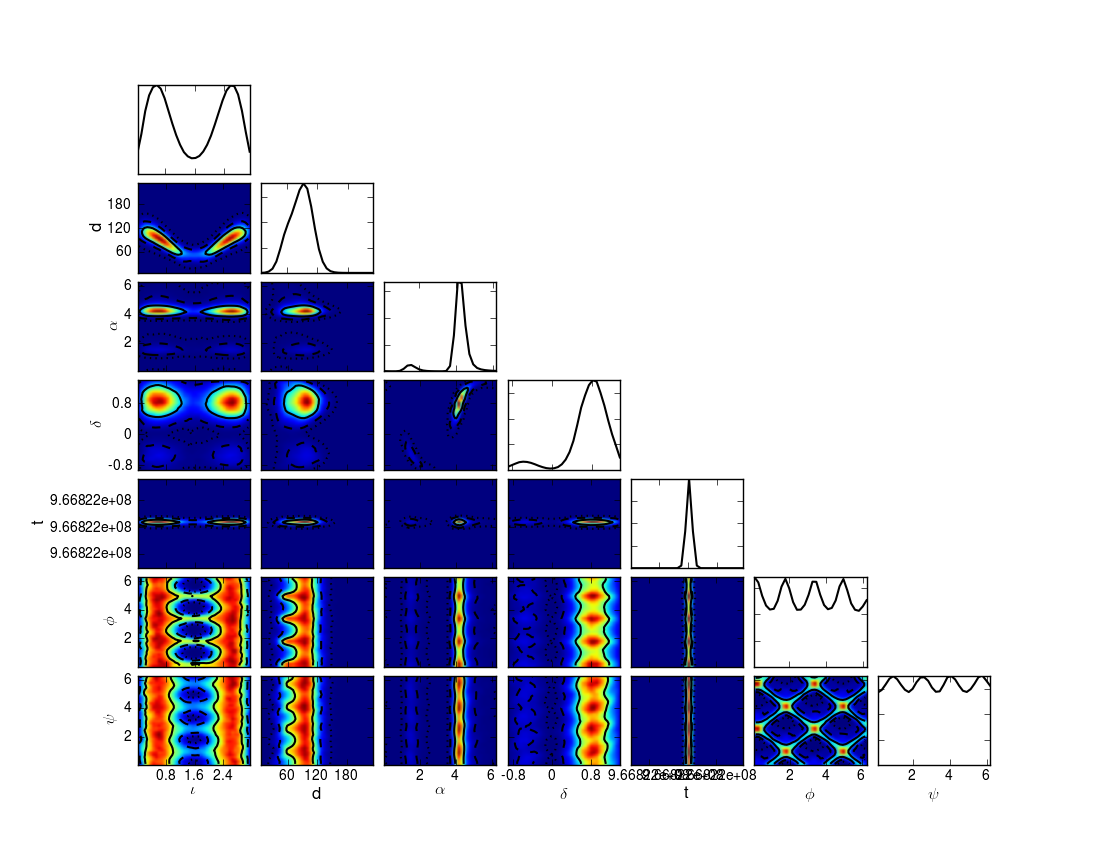
\includegraphics[width=\textwidth]{../Figures/v2runs_coinc_id_833_ILE_triplot_MASS_SET_0}
\caption{\label{fig:FiducialEvent:Triplot:TriggerMasses}\textbf{Posterior distribution in intrinsic parameters, assuming known masses}: For our fiducial event, our predicted
  distribution of extrinsic parameters $d,RA=\alpha,DEC=\delta,\iota,t,\phi,\psi$, for clarity evaluated assuming at the
  mass parameters identified by the search.  Extremely similar distributions are recovered at each mass point.   \emph{Suggest: show d-cos iota, skymap, and phi-psi only, not full triplot}
}
\end{figure*}


\begin{figure}
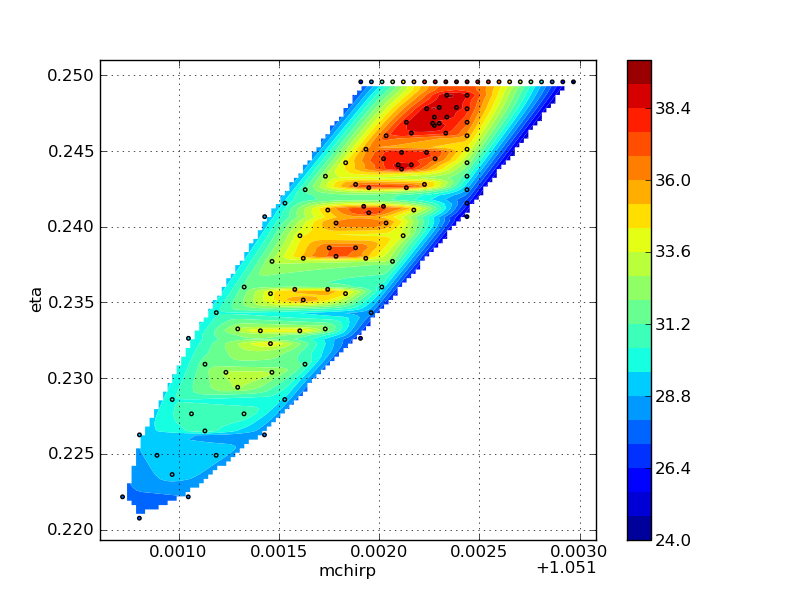
\includegraphics[width=\columnwidth]{../Figures/v2runs_coinc_id_833_mchirp_eta_logevidence}
\caption{\label{fig:FiducialEvent:LikelihoodVersusMchirpEta}\textbf{Marginalized likelihood and posterior distribution versus component masses}: \emph{Top panel}: For our fiducial event,
  contours of the log of integrated likelihood $\ln L_{\rm red}$ versus component masses, represented in $\mc,\eta$
  coordinates.  Points indicate the mass grid adopted; colors and the color bar indicate specific numerical values.   
\emph{Bottom panel}: The 90\% confidence interval derived from $L_{\rm red}$, for several noise realizations.  For
comparison, the prediction from a Fisher matrix is shown as a solid black curve.
 \textbf{PLACEHOLDER/INTENT}
}
\end{figure}



\begin{figure}
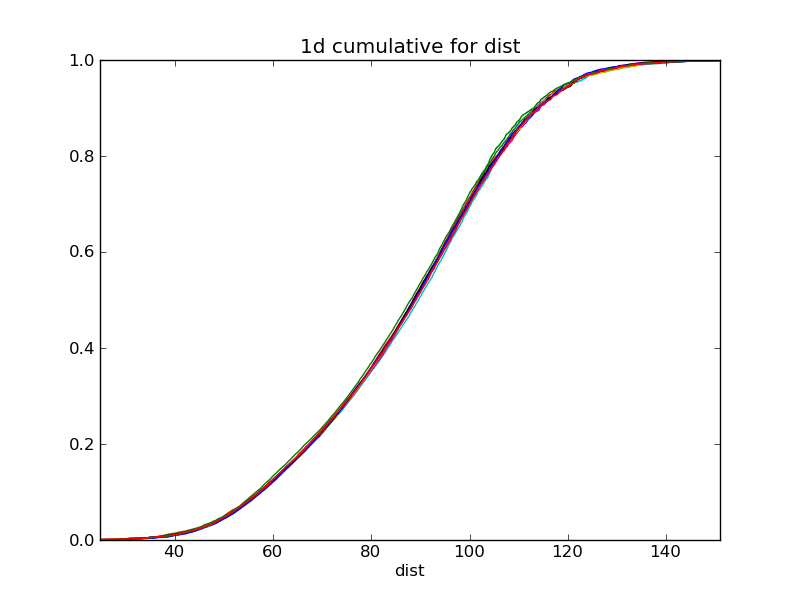
\includegraphics[width=\columnwidth]{../Figures/v2runs_coinc_id_833_cumulative-multiplot-distance-MASS_SET_0}
\caption{\label{fig:FiducialEvent:Cumulatives:Comparison:TriggerMasses}\textbf{Sampling error analysis I: One-dimensional cumulative distribution at fixed mass}:  For each of the 10 independent
  instances used at  the mass  parameters   identified by the search, a plot of the one-dimensional cumulative
  distribution in distance.  These distributions agree to within a few \textbf{(quantify)} percent, qualitatively
  consistent with a naive estimate based on $1/\sqrt{n_{\rm eff}} \simeq 4\%$.   Combining all 10
  independent runs, we expect the final distance posterior has even smaller statistical sampling error
  (\textbf{quantify} $\simeq X/\sqrt{10}$).  Our final posterior
  distributions, having support from several mass points, should have smaller statistical error still.
}
\end{figure}

\begin{figure}
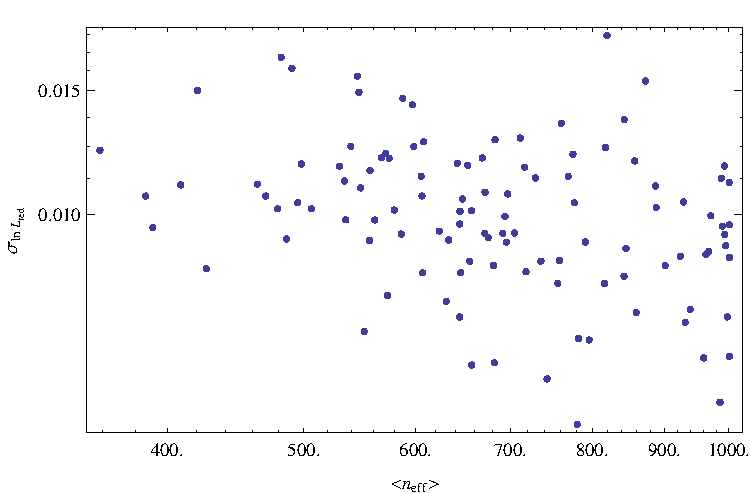
\includegraphics[width=\columnwidth]{../Figures/fig-mma-manual-v2_coinc_833-IntegralVarianceVersusNeff}
\caption{\label{fig:FiducialEvent:Integral:ErrorEstimate}\textbf{Sampling error analysis II: Integral error}: For each of the 111 mass points evaluated for the fiducial
  event, a scatterplot of the mean number of effective samples $n_{\rm eff}$ versus the standard deviation in $\ln
  L_{\rm red}$, where at each mass point the mean and standard deviation are calculated over the 10 independent
  evaluations performed.  Considering our final prediction for $L_{\rm red}$ combines all 10 events, this figure
  suggests $L_{\rm red}$ is known to better than $1\%$ for each mass point.
}
\end{figure}

\subsection{Ensemble of events}

If our estimates for the one-dimensional cumulative distributions $P(<x)$ are unbiased and if $x_*$ is a random variable
consistent with the prior, then $P(x_*)$ should be a uniformly-distributed random variable.   To test this hypothesis,
we use the one-dimensional posteriors provided by the MDC.
%% we perform repeated simulations, where each injected event was drawn from our prior:
%% \begin{itemize}
%% \item 2015 BNS MDC:   We selected \nEventsMDC{} events from the 2015 BNS MDC, identified by the GSTlal pipeline.  While all events
%%   have two-dimensional skymaps produced by \BS{}, the analysis presented below did \textbf{not} use two-dimensional skymaps.

%% While the NS-NS binaries in the 2015 MDC had generic spins, our parameter estimation model assumed zero spin.
%% \end{itemize}

% POINT: pp plots for an ensemble of events
For each parameter $x$, each colored curve in Figure  \ref{fig:pp:2015Ensemble} is  the fraction of events with
estimated cumulative probability $P(<x_*)$ at the injected parameter value $x_*$.  
Specifically, if $P(x_{*q})$ are the sorted cumulative probabilities for the $q=1\ldots n$ events with
$P(x_{*1})<P(x_{*2})$, then the points on the plot are $\{P(x_{*,q}),q/n\}$.  
%

\begin{figure}
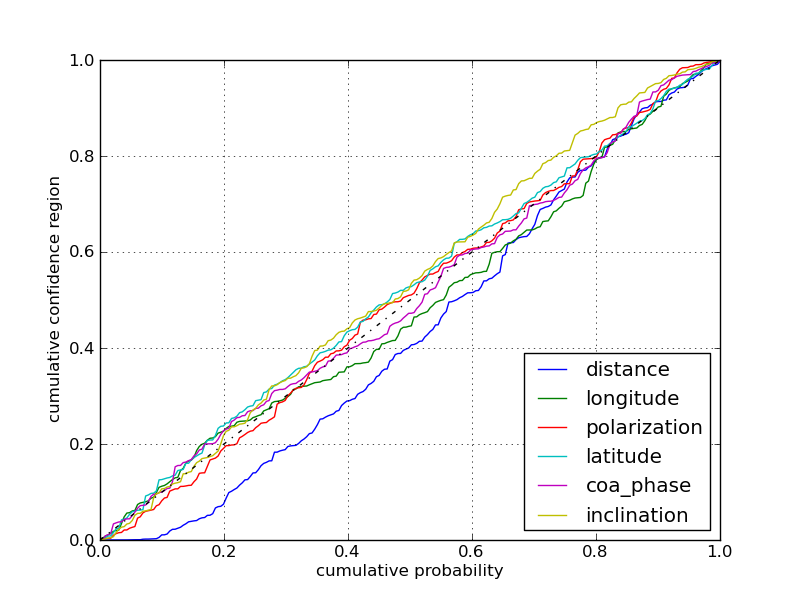
\includegraphics[width=\columnwidth]{../Figures/2015_BNS_MDC_pat_and_chris_pp_plot}
\caption{\label{fig:pp:2015Ensemble}\textbf{PP plot for ensemble of XXX NS-NS events}: \emph{Top panel}: For \textbf{X} randomly-selected NS-NS binaries, a plot of
  the cumulative distribution of $P_\theta(\theta_k)$ for each extrinsic variable $\theta=d,RA,DEC,\iota,\psi,\phi_{\rm
    orb}$.
\emph{Bottom panel}: The sky area associated with higher-probability pixels than the true sky position of the source.
}
\end{figure}


\section{Conclusions}

Conclusions go here.

\appendix


\section{Notation, definitions, and equations}

\subsection{Definitions}
\begin{itemize}
\item $\lambda$ : intrinsic coordinate, including masses and spins.

\item $\theta$ : extrinsic coordinate, including $d,RA,DEC,\iota,\psi_L,t,\phi_{\rm orb}$

\item $p_s(\theta)$: (joint) sampling prior in extrinsic dimensions

\item $p(\theta)$ : prior on extrinsic parameters

\item $L(\lambda,\theta)$ : likelihood.  In terms of individual detector strains $H_k$ and power spectra, provided by
\begin{eqnarray}
\ln L &\equiv \sum_k \ln L_k  = \ln L_{\rm model} + \ln L_{\rm data} \\
\ln L_{\rm model} &\equiv -\frac{1}{2} \sum_k \qmstateproduct{H_k}{H_k}_k  \\
\ln L_{\rm data} &\equiv  \sum_k \text{Re} \qmstateproduct{H_k}{\hat{H}_k}_k 
\end{eqnarray}

\item $Z(\lambda) \equiv L_{\rm red}(\lambda,\theta)$ : reduced or integrated likelihood, derived from $L$ via
\begin{eqnarray}
Z(\lambda) = L_{\rm red}(\lambda) = \int d\theta \; p(\theta) L(\lambda,\theta)
\end{eqnarray}

\item 
$w=Lp/p_s$ : weight

\item 
$n_{\rm eff}$ : ``effective number of samples''
\begin{eqnarray}
n_{\rm eff} \equiv  \frac{\sum_k w_k}{\text{max}_k w_k}
\end{eqnarray}

\item 
$h(t|\lambda,x)=h_+-i h_\times$ : complex gravitational wave strain

\item 
$h_{lm}(t)$: coefficients of a spin-weighted spherical harmonic decomposition
\begin{eqnarray}
\label{eq:def:hSpinWeightEmissionDirection}
h(t|\lambda,\theta) = \sum_{lm} h_{lm}(t|\lambda) e^{-2i\psi_J}\Y{-2}_{lm}(\theta_{JN}\phi_{JN})
\end{eqnarray}

\item 
$\tilde{h}(f)$ : two-sided Fourier transform of the complex function $h(t)$
\begin{eqnarray}
h(t) = \int_{-\infty}^{\infty} \frac{d \omega}{2\pi} \; e^{-i\omega t} \tilde{h}(\omega) 
\end{eqnarray}

%% \item
%% ${\cal I}$ : complex conjugation in time.  Provided to avoid confusion with $\tilde{h}^*$.  \textbf{Hopefully we won't
%%   need it.}


\item 
$\vec{x}_k$ : Position of the $k$th detector

\item 
$F_{+}$, $F_{\times},F$ : detector response function  to the $+,\times$ polarizations for sources visible in the
  $\hat{n}$ direction relative to detector
\begin{eqnarray}
F(\hat{n}) = F_+(\hat{n}) +i F_\times(\hat{n})
\end{eqnarray}

\item 
$\hat{H}_k$ : measured strain in  the $k$th detector

\item 
$H_k$ : strain response of the $k$th detector to an incident strain $h$
\begin{align}
H_k(t) &=F_{+,k}(t) h_+(t-\vec{x}_k(t)\cdot \hat{k}) + F_\times(t) h_\times(t-\vec{x}_k(t)\cdot \hat{k}) \\
 &=  \frac{F h(t-\vec{x}_k\cdot \hat{k}) }{2} + \frac{F^*h^*(t-\vec{x}_k\cdot \hat{k})}{2}
\end{align}

\item 
$S_k$ : noise power spectrum for the $k$th detector

\item 
$\qmstateproduct{a}{b}_k$ : complex-valued inner product defined by the $k$th detector's noise power spectrum:
\begin{eqnarray}
\qmstateproduct{a}{b}_k \equiv 2 \int_{-\infty}^{\infty} df \frac{[\tilde{a}(f)]^*\tilde{b}(f)}{S_h(|f|) }
\end{eqnarray}


\item 
$Q_{k,lm}(\tau)$ : complex-valued single-detector, single-harmonic ``SNR'' series
\begin{eqnarray}
Q_{k,lm}(\tau) \equiv \qmstateproduct{\exp(-i\omega \tau) h_{lm}}{\hat{H}_k}_k
\end{eqnarray}

\end{itemize}

\subsection{Other assumptions}
Assuming the earth does not rotate significantly during the signal, allowing us to approximate
\begin{eqnarray}
\qmstate{H_k} = \frac{e^{i\omega \hat{k}\cdot \vec{x}_k}}{2}\left[ 
   F_k  \qmstate{h} + F_k^* \qmstate{h^*} 
 \right]
\end{eqnarray}


\begin{widetext}
\subsection{Core equations}

\begin{align}
\ln L_{\rm data}(\lambda|t,\hat{n},\hat{k},\psi_J,d) &=  \sum_k\qmstateproduct{H_k}{\hat{H}_k}_k \nonumber \\
\label{eq:Implementation:lnLData}
&= (d_{\rm ref}/d) \text{Re} \sum_k \sum_{lm}(F_k(-\hat{k}) e^{-2\psi_J} \Y{-2}_{lm}(\hat{n}))^* Q_{k,lm}(t-\hat{k}\cdot x_k)
\end{align}

\begin{subequations}
\label{eq:ComputeRhoViaInnerProductMatrix}
\begin{align}
{ U_{k,lm,l'm'}(\lambda)}& = \qmstateproduct{h_{lm}}{h_{l'm'}}_k \\
V_{k,lm,l'm'}(\lambda)& = \qmstateproduct{h_{lm}^*}{h_{l'm'}}_k \\
\ln L_{\rm model}(\lambda|\hat{n},\hat{k},\psi_J,d) &=
   -\frac{(d_{\rm ref}/d)^2}{2}\sum_k
\left[
{
 \frac{1}{2}|F_k(-\hat{k})|^2 U_{k,lm,lm'}(\lambda)[\Y{-2}_{lm}(\hat{n})]^*\Y{-2}_{l'm'}(\hat{n})
}
 \right. \nonumber \\ & \left.
 {
+
 \frac{1}{2} \text{Re} V_{k,lm,l'm'} e^{-4i\psi_J}F_k^2 \Y{-2}_{lm}(\hat{n})\Y{-2}_{l'm'}(\hat{n})
}
\right]
\end{align}
\end{subequations}


One-dimensional marginalized posteriors, generally and sampled: 
\begin{eqnarray}
p_1(x_1|{\cal D}) dx_1 \equiv \int p(x|{\cal D}) dx = \frac{dx_1}{Z} \int dx_{2}\ldots dx_n p(x_2)\ldots p(x_n)L(x_1\ldots x_n) 
\end{eqnarray}
\begin{eqnarray}
\hat{p}_1(z) \equiv \frac{1}{N \hat{Z}}\sum_{k=1}^N K(x,x_k) \frac{L_k p_k}{p_{s,k}} 
\; ; \qquad
\hat{Z} \equiv \frac{1}{N} \sum_{k=1}^N \frac{L_k p_k}{p_{s,k}}
\end{eqnarray}
where $K(x,y)$ is some normalized ($\int K(x,y) dx = 1$) kernel  and where $\hat{Z}$ is our running
estimate for the evidence ($Z = \int L p dx$).


\end{widetext}

\section{Discrete data handling}
\label{ap:DiscreteData}
% COMPARISON: Findchirp, http://arxiv.org/pdf/gr-qc/0509116v2.pdf

In the text we describe the core algorithm using continuous time- and frequency notation, omitting most practical
details involved in operating on discrete timeseries.  In this appendix, we describe in detail the operations we perform
on discretely-sampled detector timeseries $\hat{H}_k$  and  waveform modes $h_{lm}(t)$ to calculate the likelihood
provided in the text.

\subsection{Discrete filtering}
% REQUIRED
%    - h: How we got it, and the fourier transform.
%    - frequency limits
%    - S_h and inverse spectrum truncation

% POINT: Data selection and time windows
Based on a proposed GPS geocenter event time $t_*$ and intrinsic parameters $\lambda$, we operate on all discretely-sampled detector
data $\hat{H}_k(t)$  in each instrument $k$ for the following GPS time interval:
\begin{align}
t &\in [-T_{\rm seg},T_{\rm seg}]+t_{*} \\
T_{\rm sec} &= T_h+T_{\rm spec} +T_{\rm safety} \\
T_{\rm safety} &= 2\unit{s} \\
 T_{trunc} &= 8 \unit{s} \\
T_h &= \text{waveform duration at }\lambda
\end{align}
In this expression, we compute the waveform duration $T_h$ by evaluating the simulated waveform from a starting
frequency $f_{\rm low}$ until merger. 

% POINT:
All waveform modes $h_{lm}$ are provided on a discretely-sampled time grid by \texttt{lalsimulation}.  
%
All waveform and detector-data ($\hat{H}$) timeseries are zero-padded to the next power of 2 before further operations are
performed.  
%
No windowing is performed on either the data or input waveform, either to smooth unphysical startup and termination
discontinuities in $h_{lm}(t)$ or to eliminate discontinuities between the starting and ending timesample in $\hat{H}(t)$
%
All detector and waveform data are sampled at 16384 Hz.  
%


% POINT: Two-sided fourier transform: hlmoff
The discretized fourier-transform of a complex-valued timeseries $h(t)$ on $N$  values $t_j=j\Delta t+t_0$ is
implemented as usual by the forward complex FFT:
\begin{eqnarray}
\tilde{h}(k) = \Delta t  \sum_k e^{2\pi i j k} e^{2\pi i \Delta f k t_o} h(t_j)
\end{eqnarray}
where $k=0\ldots N-1$.  Bins $k\le N/2$ correspond to positive frequencies and $k>N/2$ correspond to  negative
frequencies.    As all data segments  have the same sampling rate and cover the same time interval, we henceforth set $t_0=0$.  
% 

% POINT: PSD estimate, resampling, and inverse spectrumtruncation
We rely on other codes to assess and report on detector noise near the event.   From the recorded discrete noise power
spectrum $S_0(f)$, we construct a discrete Fourier-domain inverse spectrum filter $K(f)$ on a targeted frequency interval $|f|
\in [f_{\rm min}, f_{\rm max}]$ with frequency spacing $\Delta f$ by 
% lalsimutils.get_psd_series_from_xmldoc
% lalsimutils.resample_psd_series
(a) interpolating $1/S_0(f)$ onto a discrete frequency grid, as $K_0(f)$; 
% lalsimutils.ComplexIP : inv_spec_trunc_Q=True
(b) coarse-graining the power spectrum by performing \emph{inverse spectrum truncation} \cite{2012PhRvD..85l2006A} to construct a filter with bounded duration $T$ from $K_0$:
\begin{eqnarray}
 K =  |{\cal F} [\Theta_{T_{\rm spec}} \times {\cal F}^{-1}[ \sqrt{K_0} ]]|^2
\end{eqnarray}
where ${\cal F}$ is the fourier transform; $\Theta_T(t)$ is a step function in time which is nonzero only for $t\in[-T/2,T/2]$; and $T_{\rm spec}=8\unit{s}$ is a
constant time interval. 
%
In the frequency interval $|f|\in[f_{\rm min},f_{\rm max}]$, the discrete inverse filter $K(f)$ nearly agrees with the
input inverse spectrum $1/S_0(f)$.  Unlike the original filter, however, the inverse-spectrum-truncated filter has
support for all frequencies $f\ne 0,f_{\rm Nyq}$.     
%
To be concrete, inverse spectrum truncation is implemented precisely as previously  \cite{2012PhRvD..85l2006A}, using
real (one-sided) discrete fourier transforms: 
%
% lalsimutils.ComplexIP : inv_spec_trunc_Q=True
we populate an array of length $1+f_{\rm Nyq}/\Delta F$ with values $K_{0,q} =1/S_o(q \Delta f)$ from $q\Delta f$ between $f_{\rm min}$ and $f_{\rm max}$; 
we perform one-sided fourier transform of $\sqrt{K_{0}}$, populating a complex array of length $N=2 f_{\rm Nyq}/\Delta f$; 
we set all bins with $q\in [N_{\rm spec}, N-N_{\rm spec}]$ to zero, where $N_{\rm spec} = \floor*{T_{\rm spec}/\Delta
  T}$; 
and  finally we inverse-fourier transform and square to construct a one-sided real-valued array $K(q\Delta f)$.  
%
The two-sided filter is constructed by mirroring the original one-sided array $K$ about $f=0$, using the same packing
scheme we adopted for two-sided fourier transforms.  
%  - I don't want to discuss how lalsuite packs its FFT arrays

% POINT: Discrete filter for inner products
The inner product arrays $U_{k,lm,l'm'}$ and $V_{k,lm,l'm'}$ are constructed using this discrete filter by a discrete
approximation to the integral.  For example, the first array is evaluated as
\begin{eqnarray}
U_{k,lm,l',m'}(\tau_q) = 2 \sum_s \Delta f  K_k(f_s) \tilde{h}_{lm}^*(f_s) \tilde{h}_{l'm'}(f_s)
\end{eqnarray}
The sum includes all frequency bins, corresponding to both positive and negative frequency.  % Specifically, we do not re-impose any constraint on $f$.


% POINT: Discrete filter output
The $Q_{k,lm}(t)$ are the output of continuously filtering each detector's data against the $h_{lm}$ mode.  Using the
discrete arrays representing the fourier-domain modes $\tilde{h}_{lm}(f_q)$, data $\tilde{\hat{H}}_k(f_q)$, and inverse-noise-spectrum  $K_k(f_q)$, we estimate the
filter output via an inverse fourier transform:
\begin{eqnarray}
Q_{k,lm}(\tau_q) = 2 \sum_s \Delta f e^{+2\pi i \tau_q f_s} K_k(f_s) \tilde{h}^*_{lm}(f_s) \tilde{\hat{H}}_k(f_q)
\end{eqnarray}
%
As needed, we evaluate $Q_{lm,k}(\tau)$ for arbitrary $\tau$ by  cubic spline interpolation.  


% POINT: Finite time window?  Provided in text


\subsection{Discrete time marginalization with and without interpolation}

% POINT: What time marginalization is
The likelihood can be efficiently marginalized in time by introducing a discrete grid:
\begin{eqnarray}
\int_{t_*-T_{\rm window}/2 }^{t_*+T_{\rm window}/2}L(t) \frac{dt}{T_{\rm window}} \simeq \Delta t \sum_q e^{\ln L(t_q)}
\end{eqnarray}
where $L(t) $ is the likelihood versus time, all other parameters fixed.   
%

% POINT
We have implemented time marginalization using two approximations for the likelihood $L(t)$ versus time.  In one,  the  functions
$Q_{k,lm}(\tau)$ are evaluated using cubic spline interpolation; in the other, a method equivalent to nearest-neighbor interpolation.  For
the 16kHz data rate and signal amplitudes used, the two methods agree.   Because nearest-neighbor interpolation
corresponds to using a shifted version of the  discrete output $Q_{k,lm}(\tau_s)$ of the discrete filter, the latter
implementation is slightly faster.   
%
Unless explicitly stated otherwise, we adopt the latter method to produce all results.  


\ForInternalReference{

\section{[Internal use] Results: Targeted studies}

\begin{itemize}
\item Single event, 100 noise realizations, plus comparison with Fisher matrix

\item Zero-spin 2015 MDC: [\textbf{Not started}]  For completeness, we propose to reproduce the 2015 MDC,  using
  injections with exactly zero spin.

\end{itemize}

\subsection{Detailed investigation of one event}
Sample run results: Single event, with full DAG, done multiple times (for complete consistency/reproducibility)

Sample run results: extrinsic parameters (for one and several noise realizations)

Sample run results: $L_{\rm red}(\mc,eta)$ (for one and several noise realizations). Expected accuracy at each mass
point.. Translating into  $p(m_1,m_2)$ using a uniform mass prior.

Comparison with Fisher and MCMC


\section{[Internal use] Results: Additional production-environment investigations}

\begin{itemize}
\item 2016 BNS MDC: [\textbf{Not started}]

\end{itemize}

\section{[Internal use] Incomplete or not-yet-implemented investigations}

\subsection{Measures of convergence}

Measures to assess whether we're done
\begin{itemize}
\item * Integral: Classic MC error estimate (central limit); reproducibility across runs and via subsamples (e.g., chisquared)

\item * 1d posterior:  $n_{\rm eff}$; $L^2$ or KL divergence between subsamples or across runs

\item * sampling distribution: similarly
\end{itemize}


\subsection{Semianalytic marginalization over distance}


\section{[Internal use] Future directions}

\section{[Internal use] Patches pending or desired}

Persons/proposing supporting  a change listed as [name].

\noindent \textbf{Next push}

* Bugfix on ILE MC variance

* Uniform on sky prior with bayestar skymaps

\noindent \textbf{Minor code tweaks}

* [ROS] Larger nchunk

* [ROS] Change tempering exponent definition from $(Lp/p_s)^\beta$ to $L^\beta p/p_s$, to facilitate analysis


\noindent \textbf{Infrastructure}

* [ROS] Change DAG (number of jobs, max iterations): current solution with skymap is overkill


* [ROS] For automated end-to-end tests, add GSTlal coinc generation and \BS{} skymaps to \texttt{stage\_injections}

* [ROS] Add posterior in mchirp, eta accounting for prior.
}
\bibliography{overviewexport}
\end{document}
